\documentclass{beamer}

\mode<presentation> {

%\usetheme{default}
\usetheme{Rochester}
\usecolortheme{lily}

\setbeamertemplate{footline}[page number] 
\beamertemplatenavigationsymbolsempty
\setbeamertemplate{bibliography item}{} %Remove icons in bibliography
}

\usepackage{graphicx} % Allows including images
\usepackage{amsmath}
\usepackage{lmodern}
\usepackage{listings}
\usepackage{hyperref}
\usepackage{wrapfig}



\usepackage{tikz}
\usetikzlibrary{bayesnet}

\lstset{
    language=[5.0]Lua,
    basicstyle=\fontsize{11}{9},
    sensitive=true,
    breaklines=true,
    tabsize=2
}

%----------------------------------------------------------------------------------------
%	TITLE PAGE
%----------------------------------------------------------------------------------------

\title[SGVB_topic]{SGVB Topic Modelling} 

\author{Otto Fabius} 
\institute[UvA] 
{University of Amsterdam \\
Supervisor: P.Putzky \\ 
Co-Supervisors: M. Welling, D.P. Kingma
\medskip
}
\date{\today} % Date, can be changed to a custom date

\begin{document}

\begin{frame}
\titlepage % Print the title page as the first slide
\end{frame}


%----------------------------------------------------------------------------------------
%	PRESENTATION SLIDES
%----------------------------------------------------------------------------------------

\section{LDA}


\begin{frame}
\frametitle{Latent Dirichlet Allocation (LDA)}
\begin{wrapfigure}[0]{r}{0.5\textwidth}
  \centering
    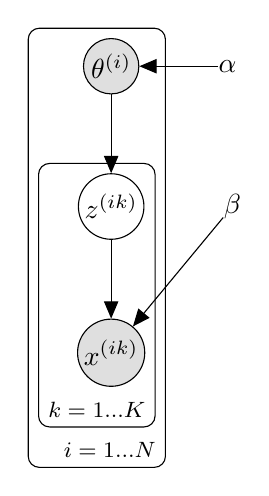
\begin{tikzpicture}[node distance = 1.5cm]
        \node[obs] (x) {$x^{(ik)}$}; 

        \node[latent, above=of x] (z) {$z^{(ik)}$}; 
        
        \node[obs, above=of z] (d) {$\theta^{(i)}$}; 

        \node[const, right=of d] (a) {$\alpha$} ;
        \node[const, right=of z] (th) {$\beta$} ;
		
		\edge {a} {d};
        \edge {z} {x};
        \edge {d} {z};
        \edge {th} {x};

		
		\plate {xz} {(x)(z)} {$k = 1...K$};
        \plate {xzd} {(x)(z)(d)(xz)} {$i = 1...N$};
	  
    \end{tikzpicture}

\caption{Graphical Model of LDA}
\label{lda}
\end{wrapfigure}
- Generative model\\
- Dirichlet priors\\ 
- $\theta^i$ and $z^{(ik)}$ model topic,\\
\hspace{5mm} both multinomials \\
- $z^{(ik)}$ drawn from $\theta^{(i)}$,\\
\hspace{1.6mm} $x^{(ik)}$ drawn from $z^{(ik)}$\\
\vspace{40mm}
\end{frame}

\begin{frame}
\frametitle{Graphical model}
\begin{figure}[ht]
  \begin{center}
    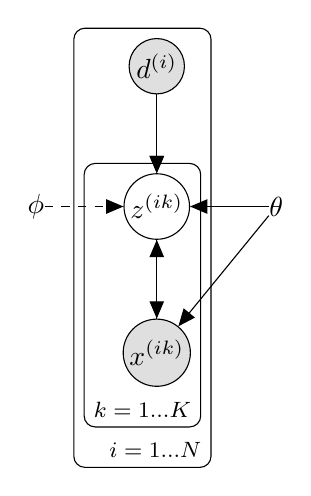
\begin{tikzpicture}[node distance = 1.5cm]
        \node[obs] (x) {$x^{(ik)}$}; 

        \node[latent, above=of x] (z) {$z^{(ik)}$}; 
        
        \node[obs, above=of z] (d) {$d^{(i)}$}; 

        \node[const, right=of z] (th) {$\theta$} ;
        \node[const, left=of z] (ph) {$\phi$};

        \edge {z} {x};
        \edge {d} {z};
        \edge {th} {z};
        \edge {th} {x};

        \edge [dashed] {ph} {z}
        \edge [dashed,bend right] {d} {z}
        \edge [dashed,bend left] {x} {z}
		
		\plate {xz} {(x)(z)} {$k = 1...K$};
        \plate {xzd} {(x)(z)(d)(xz)} {$i = 1...N$};

    \end{tikzpicture}
  \end{center}
\caption{Graphical Model of SGVB Topic Modelling}
\label{sgvb_topic}
\end{figure}

\end{frame}



\end{document}